\chapter{Conclusion and Future Directions}
\label{chap:conclusion}
% Discussion: remaining challenges, the benefits in another fields than oncology

My dissertation contributes to a better toolbox for cancer proteogenomic and multi-omics characterization and generates insights into glioblastoma disease biology that will lead to novel therapeutic avenues. In \Cref{chap:mut-pipeline-qc}, we investigated the data harmonization using standardized data processing pipelines on establish bulk genomic sequencing technologies. Data harmonization is part of the critical infrastructure of large-scale multi-omics studies to ensure the generated datasets can be integrated with other data of interest and re-used by the research community. We showed that the data harmonization on Genomic Data Commons is applicable to various studies across cancer types. More importantly, the harmonized outputs do not significantly alter the downstream biological findings and interpretation. In the cases where technical artifacts are introduced, those artifacts are carefully characterized and documented. Pipelines on GDC have since been applied to more cancer projects. Other data commons of different data types are actively being developed, including Proteomic Data Commmons and Imaging Data Commons, by following the example set by GDC.

In \Cref{chap:ptmcosmos}, we developed a database, PTMcosmos, that collects the existing knowledge of post-translation modifications in cancer and used the integrated information of PTmcosmos to analyze the experiment datasets from Clinical Proteomic Tumor Analysis Consortium to showcase its potential values to the research community. We collected the proteomic datasets from CPTAC, a consoritum with the goal of proteogenomic multi-omics characterization of patient tumors across multiple cancer types. By harmonizing the CPTAC's mass spectrometry based global protein and PTM abundance measurements with existing supporting evidences of PTM sites, we were able to identify pan-cancer PTM dysregulation events that are not explained by the known upstream genetic alterations or associated with clinically relevant tumor subtypes. We also investigated the mutational impact on PTM through protein structure guided spatial clustering. Furthermore, the easy-to-use user interface of PTMcosmos brings such functionalities to the end user, allowing the broader research community to utilize the immense amount of new PTM information brought by CPTAC and the known functions and annotations of PTMs from the literature.

In \Cref{chap:cptac-gbm-discov}, we focused on the proteogenomic characterization of glioblastoma deadly brain tumor without personalized treatment as a CPTAC study. During the data analysis, we utilized the ``toolbox'', where the genomic data were harmonized on GDC and PTM annotations were pulled from PTMcosmos. Our analysis contributes to the potential improvement of patient stratification and discovery of new therapeutic options. Using multi-omics clustering, we identified a subset of patients with mixed subtypes compared with traditional sequencing-based subtypes, who exhibit shortened overall survival. Phosphoproteomic data indicate that PLCG1 and PTPN11 act as a common signaling hub for multiple RTKs. Given the high RTK genetic alteration frequencies and eventual remission in GBM, a combined therapy targeting both RTKs and their shared signaling hub might be more effective. Using connectivity map approach, we identified some druggable targets based on the gene and protein signatures of GBM tumors. By integrating the bulk multi-omics with single cell transcriptomics, we dissected the tumor microenvironment and characterized the immune composition differences and the potential signaling transduction regulation. In sum, our findings bring new insights towards a better understanding of GBM and hopefully a better personalized treatment for GBM patients.


new pipelines for new technology

gene annotation unification MANE

pan-cancer PTM
- reprocess the data
- kinase substrate library



With the map of \fref{fig:gbm-graphical-abstract}

longitudal study

overview of the next gbm confirmatory cohort

\begin{figure}[tb]
    \centering
    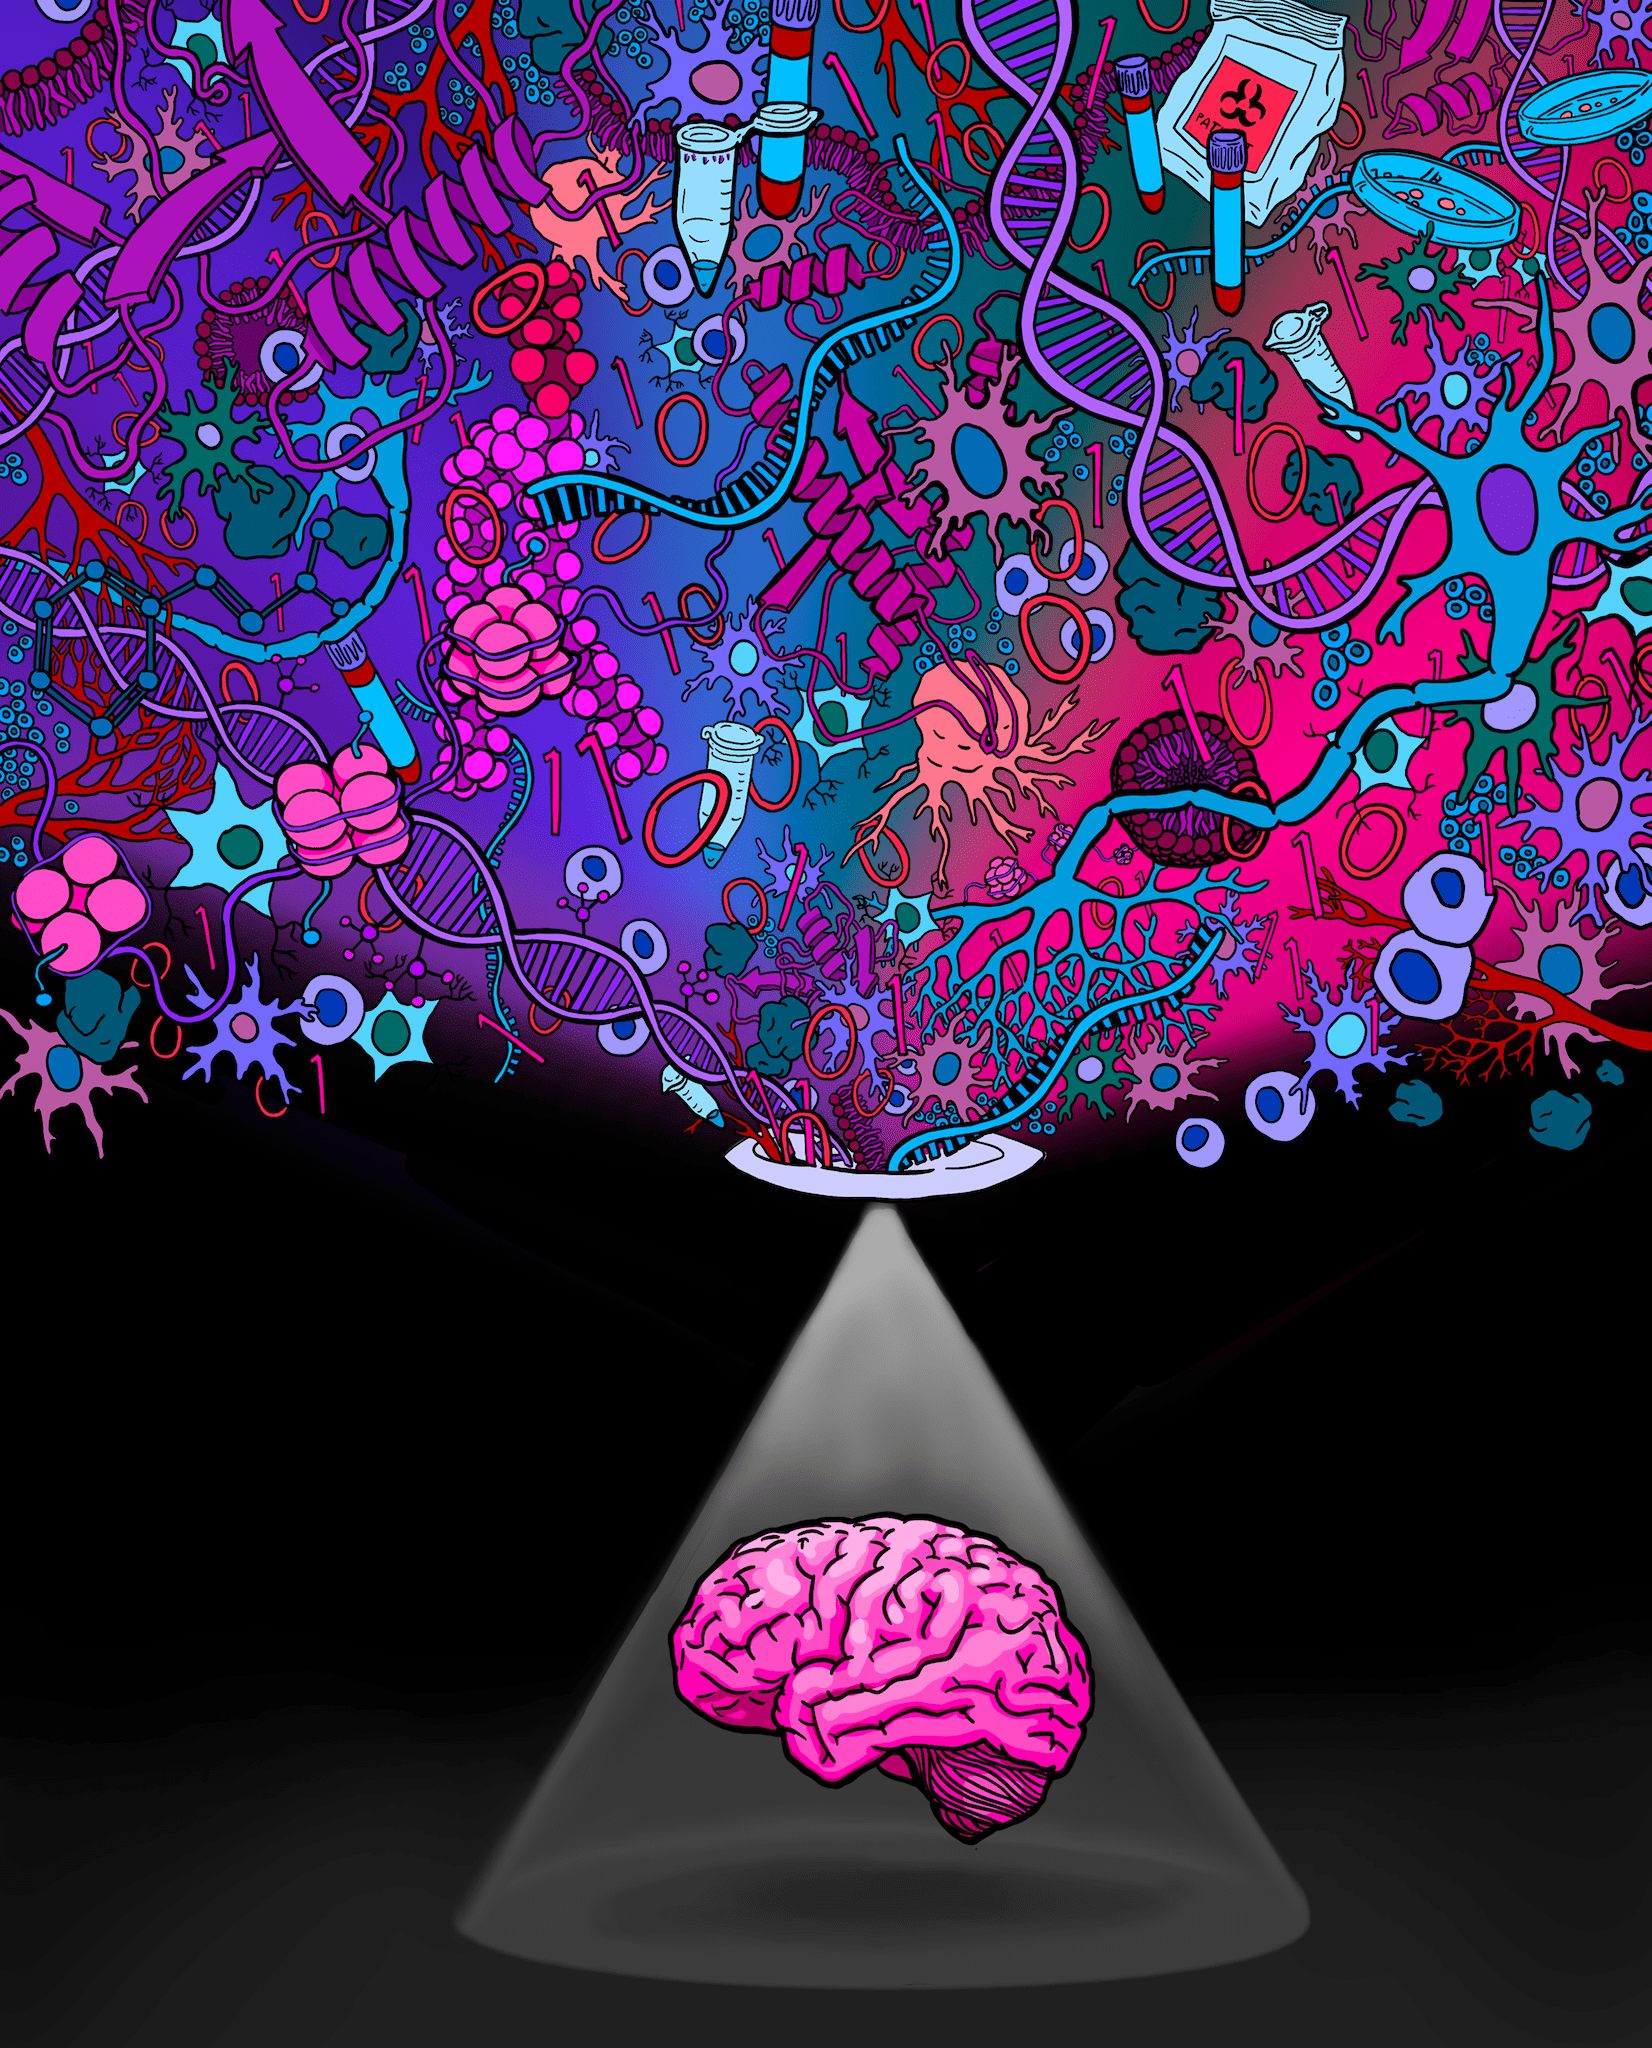
\includegraphics[width=0.6\linewidth]{figures/chap05_conclusion/cptac_gbm_cancer_cell_cover.png}
    \caption[Better disease understanding through a lens for an integrative view of multi-omics datasets.]{Better disease understanding through a lens for an integrative view of multi-omics datasets. Cover art of \textit{Cancer Cell} (April 2021 issue). Artwork by Jessica Johnson \url{https://jessicajohnsonart.com/}.}
    \label{fig:lens-multi-omics}
\end{figure}

\begin{figure}[tb]
    \centering
    \phantomlabel{fig:cptac-gbm-future-plan-longitudinal}
    \phantomlabel{fig:cptac-gbm-future-plan-heterogeneity}
    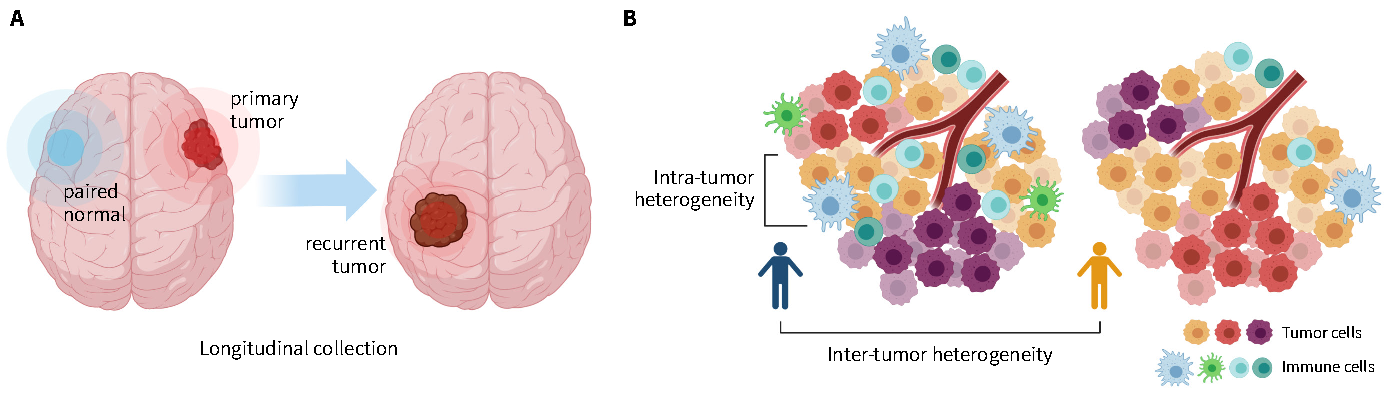
\includegraphics[width=1\linewidth]{figures/chap05_conclusion/gbm_future_plan.pdf}
    \caption[CPTAC GBM study future plan.]{%
        CPTAC GBM study future plan.
        \subref{fig:cptac-gbm-future-plan-longitudinal} Longitudinal collection of tumor samples and paired normal samples.
        \subref{fig:cptac-gbm-future-plan-heterogeneity} Tumor heterogeneity using single cell technologies.
    }
    \label{fig:cptac-gbm-future-plan}
\end{figure}
